\documentclass{abnt}

%Arquivo com os principais pacotes usados e suas descrições.

%%%%%%%%%%%%%%%%%%%%%%%%%%%%%%%%%%%%%%%%%
% 			Idiomas e Acentos			%
%%%%%%%%%%%%%%%%%%%%%%%%%%%%%%%%%%%%%%%%%
\usepackage[brazil]{babel} % Habilita o uso do idioma português do brasil (PT-BR).
\usepackage[T1]{fontenc} 
%\usepackage{fontspec} % Habilita maior variedade de acentos. Pode ser necessario adicionar outros pacotes.
\usepackage{lmodern} % Habilita o uso da font Latin Modern.


%%%%%%%%%%%%%%%%%%%%%%%%%%%%%%%%%%%%%%%%%
% 				TABELAS					%
%%%%%%%%%%%%%%%%%%%%%%%%%%%%%%%%%%%%%%%%%
\usepackage{tabulary} % Cria tabelas mais facilmente.
\usepackage{booktabs} % Melhora o visual das tabelas.
\usepackage{table}{xcolor} % Pacote de cor pra as tabelas.
\usepackage{caption} % Melhora as legendas de imagens, tabela etc.

%%%%%%%%%%%%%%%%%%%%%%%%%%%%%%%%%%%%%%%%%
% 				IMAGENS					%
%%%%%%%%%%%%%%%%%%%%%%%%%%%%%%%%%%%%%%%%%
%\usepackage{graphicx} % Facilita a inserção de imagens.


%%%%%%%%%%%%%%%%%%%%%%%%%%%%%%%%%%%%%%%%%
% 			CÓDIGO FONTE				%
%%%%%%%%%%%%%%%%%%%%%%%%%%%%%%%%%%%%%%%%%
%Documentação de código fonte.
\usepackage{listings}


%%%%%%%%%%%%%%%%%%%%%%%%%%%%%%%%%%%%%%%%%
% 	Símbolos e Caracteres Matemáticos	%
%%%%%%%%%%%%%%%%%%%%%%%%%%%%%%%%%%%%%%%%%
\usepackage{amsmath}
\usepackage{amssymb}
\usepackage{amsfonts}
%\usepackage{mathspec} %Habilita o uso das fontes e dos caracteres matematicos.


%%%%%%%%%%%%%%%%%%%%%%%%%%%%%%%%%%%%%%%%%
%				ABNT					%
%%%%%%%%%%%%%%%%%%%%%%%%%%%%%%%%%%%%%%%%%
%\usepackage[alf]{abntcite} % Ordena as referencias em ordem alfabética.
\usepackage{url} %Facilita o uso de url. Pode-se usar o comando \url{...}.


%%%%%%%%%%%%%%%%%%%%%%%%%%%%%%%%%%%%%%%%%
% 			Configurações				%
%%%%%%%%%%%%%%%%%%%%%%%%%%%%%%%%%%%%%%%%%
\captionsetup{justification=centering,labelfont=bf} %Formata a legenda das figuras.
%\graphicspath{{../imgs/}} %Define o diretorio padrão para buscar as imagens da apresentação.  
%\setromanfont[Ligatures=TeX]{Crimson}
%\defaultfontfeatures{Scale=MatchLowercase, Mapping=tex-tex}

%%%%%%%%%%%%%%%%%%%%%%%%%%%%%%%%%%%%%%%%%
%				BEAMER					%
%%%%%%%%%%%%%%%%%%%%%%%%%%%%%%%%%%%%%%%%%
%Define algumas configurações que serão validas para todo o documento.  
\setbeamertemplate{section in toc}[sections numbered]
\setbeamertemplate{subsection in toc}[subsections numbered]
\setbeamertemplate{background canvas}[vertical shading][bottom=blue!3,top=blue!7]
\setbeamertemplate{caption}[numbered]


%%%%% Dados para criação da capa e folha de rosto %%%%
\autor{	Denis F. de Carvalho, 
		Guilherme A. de Macedo, 
		Matheus L. Domingues da Silva e 
		Victor H. Carlquist da Silva
}
\titulo{Sistema Seis Sigma de Produção}
\orientador{Avelino Bazanella Junior}
\comentario{Trabalho apresentado ao Prof. Avelino Bazanela Junior, na disciplina de Administração 
			presente no $2^{a}$ modulo do curso de Tecnologia em Análise e Desenvolvimento de Sistemas no IFSP-CJO.}
\instituicao{Instituto Federal de Educação, Ciência e Tecnologia de São Paulo -- \textit{campus} Campos do Jordão}
\local{Campos do Jordão}
\data{\today}

\begin{document}

	% Para utilizar o formato padrão de capa da ABNT, substituí o comando \maketitle pelo comando \capa.
	\capa
	
	\folhaderosto
	
	\begin{resumo}
		Este trabalho tem por objetivo mostrar e explicar o funcionamento do programa Seis Sigma. A construção 
		desse trabalho foi baseada em pesquisas em \textit{sites} especializados, gráficos e tabelas, bem como a consulta 
		de livros especializados.
	\end{resumo}

	\begin{abstract}
			This work aims to show and explain the workings of the Six Sigma program. The construction of this work 
			was based on research on specialized sites, graphs and tables, and consultation of specialized books.
	\end{abstract}
	
	\sumario
	
	\listadetabelas
	
	\listadefiguras
	
	\chapter {Introdução}
	
	Seis Sigma (six-sigma ou $\sigma$-seis) é um programa de melhoria de processo baseado numa 
	metodologia de solução de problemas composto por cinco etapas: Definição, Medição, Análise, 
	Melhoria e Controle. Em sua forma mais geral, o Seis Sigma é uma forma de avaliar os níveis 
	de produção de uma empresa. O Seis Sigma foi inicialmente desenvolvido visando a melhoria nos 
	processos de manufaturas, porém hoje é utilizado pelas empresas em quaisquer tipos de processos, 
	incluindo até os processos de TI (Tecnologia da Informação).
	
	O conceito do Seis Sigma é estabelecer uma métrica universal para medir os defeitos de um processo. 
	Essa métrica estabelece que quanto mais alto o nível de sigma, melhores serão os produtos produzidos, 
	porém quanto menor for o nível de sigma, maior será a quantidade de produtos ruins produzidos pela empresa.
	
	\chapter {História}
	
	O Seis Sigma foi inicialmente desenvolvido pela Motorola.
	
	\chapter {Níveis de Sigma}
		\section {Introdução}
			O sigma é utilizado para medir a variância de qualquer processo. Os níveis de sigma medem o desempenho do processo de uma empresa.
			Geralmente uma empresa adota níveis 3 ou 4 do sigma, que são níveis considerados normais.
			
			O sigma ($\sigma$) é calculado pela seguinte fórmula: 
			\begin{center}
			    \begin{equation}
			       Z = \frac{x - \mu}{\sigma}
		        \end{equation}
		     	\begin{itemize}
		     		\item[$x$] ponto que se deseja converter em $Z$;
		     		\item[$\mu$] média da normal original;
		     		\item[$\sigma$] desvio padrão da normal original.
		     	\end{itemize}
			\end{center}
			
			 
		\section {Níveis de Qualidade}
		    Cada nível de sigma possuí um limite de desvios (problemas), que é medido em  \textit{Problemas por Milhão} (PPM) 
			\begin{itemize}
			    \item {1 Sigma}
			        \subitem O 1 Sigma tolera até 697700 (PPM), possuindo um fator de sucesso do processo de 30,23\%. 
			    \item {2 Sigma}
			        \subitem O 2 Sigma tolera até 308700 (PPM), possuindo um fator de sucesso do processo de 69,13\%.
			    \item {3 Sigma}
			        \subitem O 3 Sigma tolera até 66810 (PPM), possuindo um fator de sucesso do processo de 93,32\%.
			    \item {4 Sigma}
			        \subitem O 4 Sigma tolera até 6210 (PPM), possuindo um fator de sucesso do processo de 99,379\%.
			    \item {5 Sigma}
			        \subitem O 5 Sigma tolera até 233 (PPM), possuindo um fator de sucesso do processo de 99,9767\%.
			    \item {6 Sigma}
			        \subitem O 6 Sigma tolera até 3,4 (PPM), possuindo um fator de sucesso do processo de 99,99966\%.
			\end{itemize}
			
			Dessa forma os níveis de qualidade do sigma podem ser melhores visualizados com base na tabela a seguir:
			\begin{table}[h]
				\centering
				\rowcolors{2}{gray!10}{white}

				\begin{tabular}{rcr}
					\toprule
					Sigma & Problemas por Milhão (PPM) & Porcentagem (\%) \\
					\midrule
					 1 & 697700	& 30,23 	\\
					 2 & 308700 & 69,13 	\\
					 3 & 66810 	& 93,32 	\\
					 4 & 6210 	& 99,379 	\\
					 5 & 233 	& 99,9767 	\\
					 6 & 3,4 	& 99,99966 	\\
					\bottomrule		
				\end{tabular}
	
				\label{tab_niveisSigma}
				\caption{Níveis de Sigma.}
				
			\end{table}

		\section {Curva Normal} 
			Todo processo possui uma variação, assim como os objetos fabricados, nenhum objeto é igual ao outro, mas é preciso estabelecer um limite de variação aceitável para cada objeto.
			
			A curva de nível criada por Carl Gauss permite prever a probabilidade de um desvio ocorrer. A curva de desvios, curva normal ou curva de probabilidades de Gauss é dividida, geralmente, em três partes:
			\begin{itemize}
				\item {Limite de especificação menor}
					\subitem Probabilidade de 10\% do valor real estar nesse intervalo. 
				\item {Significativo}
					\subitem Ápice da curva, probalibidade de 90\% do valor real estar próximo a linha. 
				\item {Limite de especificação maior}
					\subitem Probabilidade de 10\% do valor real estar nesse intervalo.
			\end{itemize}
<<<<<<< HEAD
			
			\begin{figure}[h]
				\centering
				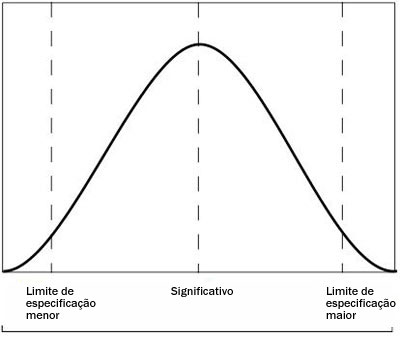
\includegraphics[width=7cm, keepaspectratio]{img/curva.jpg}
				\label{fig_curva}
				\caption{Curva Normal}
			\end{figure}
		    
=======
			\begin{figure}[h]
				\centering
				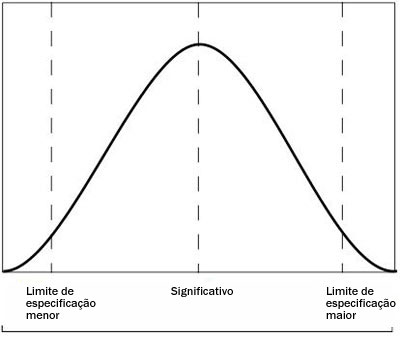
\includegraphics[width=8cm, keepaspectratio]{img/curva.jpg}
				\caption{Curva Normal.}
			\end{figure}
	    
>>>>>>> c7078ebb81cbf81f723a5633e0062ae73491b144
		\section {Vantagens do 6 Sigma}
		
		As principais vantagens do 6-sigma são: 
		\begin{itemize}
			\item {Aumento no lucro}
			\item {Diminuição de consumo de recursos da empresa}
			\item {Melhor qualidade nos produtos e/ou serviços}
			\item {Maior satisfação do cliente}
		\end{itemize}
		
		Muitas empresas com sigma entre 3 e 4 gastam em torno de 25\% a 40\% de seus recursos para resolver problemas. Com o uso do 6-sigma, esse gasto se torna lucro.
		  
				
	\chapter {Metodologias}
		\section {Introdução}
		
			 O 6-Sigma é composto, basicamente, por duas metodologias, o DMAIC e o DMADV. A diferença entre 
			 essas duas metodologias está ligada à realidade de seus processos. Novos processos utilizarão 
			 a metodologia DMADV, enquanto processos que já existam implementariam o DMAIC.
			 
			 A implementação dessas metodologias é tarefa do \textit{Master BlackBelt}, \textit{BlackBelt} e do \textit{GreenBelt}. Somente profissionais 
			 credenciados com essas patentes estão qualificados elaborarem esse tipo de projeto.
			 
			\section {DMAIC}
				O DMAIC é um acrônimo em inglês para as seguintes etapas a serem trabalhaas em 
				um processo já existente: Definir (\textit{Define}), Medir (\textit{Measure}), 
				Analisar (\textit{Analyse}), Melhorar (\textit{Improve}) e Controlar (\textit{Control}).
				\\
				A seguir mostraremos detalhadamente cada uma dessas etapas.
				
				\subsection {Definir}
					Compreende definir quais os problemas a serem tratados dentro de um determinado processo.
					\subsubsection {Objetivo}
					O obetivo da fase de definição é deixar claro o propósito do projeto. É preciso que todos
					saibam o que pode ser melhorado e o que não pode. Isso é fundamental para que falsas espectativas 
					não sejam criadas, o que geraria muitas frustações quando o projeto fosse concluído. Isso é 
					realizado determinando as espectativas do projeto de forma clara e unívoca.
					\subsubsection {Entendendo o processo}
					É um conceito fundamental da metodologia 6-Sigma que o foco tem que ser no processo
					quando um pradrão de qualidade não é atingido.\\
					Para que as melhorias sejam identificadas é preciso entender o processo.  
					É fundamental que essa etapa seja realizada com muito cuidado, pois é justamente nessa
					fase que serão identificados os problemas.
				\subsection {Medir}
					Já de posse dos documentos relativos aos objetivos, às espectativas e identificadas 
					possibilidades de melhorias em um ou mais processos, é chadada a hora de utilizar números 
					e gerar gráficos contendo as projeções e metas.
					\subsubsection {Objetivo}
					O objetivo dessa etapa é obter o máximo de informação sobre uma determinada tarefa, 
					o quão eficiente ela é e o quão eficiente ela pode se tornar. Essa etapa envolve, 
					basicamente, três tarefas: mapear o processo, coletar os dados e analisar os dados coletados.
					\\
					Falaremos dessas três tarefas separadamente.
					\subsubsection {Mapeando processo}
					O objetivo principal dessa tarefa é criar um mapeamento detalhado do processo existente.
					Não é nessa tarefa que são postas ideias sobre o que deveria ser feito de diferente. 
					Nessa tarefa, simplesmente, elaboramos um mapa do processo, seja ele do jeito que for: bom ou ruim.
					É de extrema importância, nessa fase, que sejam mapeadas todas as variações no modo como o processo é realizado e 
					nunca supor que o processo sempre realiza suas etapas da mesma maneira.
					\\
					Depois dessa tarefa realizada, ficará fácil termos uma noção dos problemas que envolvem determinado processo.
					\subsubsection {Coletando os dados}
					Depois de o problema ser identificado e termos uma visão clara do que precisamos melhorar, passamos para a 
					fase de coleta de dados. Todos os dados referentes àquele processo que queremos melhorar é coletado.
					\\
					Coletar os dados não é, comumente, uma tarefa difícil. A maioria dos processos geram informações que 
					ficam armazenadas em algum banco de dados. Em casos muito específicos é preciso que seja realizada uma 
					tarefa adicional, como, por exemplo, compilar dados que estejam muito segmentados.
					
					\subsubsection {Analisando os dados coletados}
					Essa tarefa é composta, basicamente, de gráficos e diagramas que ilustram de forma bastante clara e óbiva 
					o funcionamento do processo, gerando uma representação visual de todo o processo que se deseja melhorar. O tipo de dado vai determinar qual 
					ferrameta será usada para a representação (gráficos, diagramas ou outro método).
					\subsubsection {Calculando o nível de Sigma}
					A metodologia 6-Sigma vem do fato de que, em seu nível mais alto (o nível 6), espera-se um índice de 
					defeito de 3.4 por milhão de oportunidades (3.4 DPMO). Mas muitos projetos de 6-sigma não conseguem 
					atingir, logo de início, esses números. Essa fase visa definir qual o nível de Sigma tangível para o 
					processo em questão.
				\subsection {Analisar}
					Identificar a causa raiz dos problemas. Essa fase procura pela causa do problema.
					\subsubsection {Objetivo}
					O objetivo é identificar o problema raiz, ou seja, tentar encontrar o que está causando o problema 
					e, posteriormente, confirmar o problema com dados.\\
					Duas perguntas que devem ser respondidas durante essa fase são: "Por que o problema está acontecendo?" e 
					"O que está causando o problema?"
					\subsubsection {Causa raiz}
					É claro que as fases Definir e Medir já deram uma noção dos fatores que estão afetando a performance do processo. 
					Pode-se ter descoberto que o problema acontece em um grupo isolado onde é causa é o uso de equipamento antiquado. 
					Ou pode-se ter chegado a conclusão de que o problema é óbvio pois o processo atrasa porque é ineficiente. 
					Mas o objetivo da fase de analise é identificar o problema raiz, isso significa que deve-se ir mais fundo 
					do que apenas analisar superficialmente. Além disso, em todas as etapas do DMAIC, suspeitas e 
					hipóteses devem ser confirmadas com dados. Não basta identificar o problema, é preciso demonstrar através de números 
					que mudanças em determinados fatores impactariam substancialmente nos resultados.
					\subsubsection {Diagrama de causa e efeito}
					Depois de compilada uma lista com todas as potenciais causas-raiz é hora de organizá-las de um forma que fique 
					fácil priorizar e acessá-las.
					Nessa fase são usadas algumas ferramentas, as mais comuns são o Diagrama de Espinha de Peixe ou o Diagrama de Árvore 
					que tem o mesmo objetivo do Espinha de Peixe.\\
					O Diagrama e Espinha de peixe tem seu desenho parecido com uma espinha de peixe e serve para 
					categorizar causas potencias e ilustrar em quais níveis elas estão.
				\subsection {Melhorar}
				Nesta fase, supõe-se que o problema já esteja claro. Agora é hora de imaginar soluções, avaliar e 
				selecionar soluções e colocá-las em prática.
					\subsubsection {Objetivo}
					O objetivo para essa fase é identificar a solução para o problema. Isso envolve: 
					Imaginar alguma solução, escolher uma solução para teste, avaliar os resultados da solução aplicada.
					Normalmente uma solução piloto é aplicada para analisar os resultados, antes de aplicá-la em larga escala.
					\subsubsection {Identificando a solução}
					Identificar soluções é uma tarefa que envolve não somente a equipe do projeto como também com todos que trabalham no processo. 
					Nessa fase são imaginadas possíveis solução que contrapõem as causas-raizes encontradas na fase de Análise.
					Uma coisa importante nessa fase é que nenhuma ideia seja julgada ou descartada de primeira, mesmo aquelas que, aparentemente, não sejam 
					possíveis de implementar, pois ainda que não seja possível implementar, talvez possa ser o fio condutor para a solução.
					\subsubsection {Selecionando a solução}
					O objetivo principal dessa etapa é encontrar uma solução utilizando meios objetivos, e não soluções 
					baseadas em suposições ou preferências. Toda a metodologia 6-Sigma é baseada justamente nisso.
					\subsubsection {Implementando a solução}
					Durante a fase de implementação da solução a equipe deve monitorar o processo e anotar qualquer problema que surgir.
					Os dados devem ser revistos periodicamente para se ter certeza de que os procedimentos estão sendo seguidos.
					\subsubsection {Avaliando as melhorias}
					Na fase de avaliação de melhorias é comum implementar, primeiramente, um projeto piloto, antes de aplicar a solução 
					em larga escala. O befício de se utilizar um projeto piloto está no fato de que será mais fácil avaliar os resultados. 
					Se os resultados avaliados forem positivos, a equipe poderá aplicá-la em larga escala com uma segurança maior.
				\subsection {Controlar}
					\subsubsection {Objetivo}
					O objetivo principal da fase de Controle é assegurar que as melhorias efetuadas no processo sejam 
					mantidas até final do processo. Para isso é preciso padronizar e documentar os procedimentos.
					\subsubsection {Padronizando e documentando}
					Nessa fase documenta-se e padroniza-se todas as melhorias que foram feitas na fase de Molhorias.
					A equipe de projeto tem que ter certeza de que todos os envolvidos no processo receberam treinamento correto 
					O treinamento pode ser um curso em uma sala de aula, ou simplesmente a distribuição da documentação do processo.
					\subsubsection {Monitorando o processo}
					A fase mais crítica da etapa de controle é estabelecer um plano para monitoramento do processo. Isso é estremamente 
					necessário para se ter certeza de que o ganho adquirido será mantido. Durante essa fase é especificado quem será 
					notificado quando alguma coisa der errado e a quem essa pessoa deverá se reportar.
					Gráficos controlando o processo devem ser capazes de avisar quando alguma coisa está dando errada por meios de 
					avisos coloridos: verde para indicar que tudo está correto, amarelo para avisar que algo está perto de sair dos limites estabelecidos, 
					e vermelho para avisar que algo está fora dos limites estabelecidos.
			\section {DMADV}
				O DMADV é um acrônimo em inglês para as seguintes etapas a serem trabalhaas em um 
				novo processo: Definir (\textit{Define}), Medir (\textit{Measure}), 
				Analisar (\textit{Analyse}), Projetar (\textit{Design}) e Verificar (\textit{Verify}).
				O propósito do DMADV é criar um processo que seja eficiente desde sua concepção, já que engloba a 
				construção de um processo que ainda não existe.
				\\
				A seguir mostraremos detalhadamente cada uma dessas etapas.
				\subsection {Definir}
				A etapa de definição do DMADV é igual a etapa de definição do DMAIC. Leva-se em conta os mesmos fatores.
				O que muda é o foco. Enquanto o DMAIC define objetivos para um processo que já está em funcionamento, 
				a fase de definição do DMADV é focada em um processo que ainda não existe. Então, ao invés de se definir 
				melhorias para um processo em execução, aqui a equipe do projeto vai definir o quão bom o processo será desde 
				o seu nascimento.
				\subsection {Medir}
				Nessa etapa o foco é medir as expectativas e necessidades dos clientes. Tudo é voltado para 
				entender as necessidades do cliente e como será atendida a necessidade do mesmo.
				Priorizar as necessidades dos clientes é uma tarefa fundamental nessa etapa.
				Com base nisso, consegue-se mensurar e determinar as necessidades e especificações do novo processo.
				\subsection {Analisar}
				Analisar opções disponíveis para se atingir as expectativas dos clientes. Cria-se conceitos de projetos baseados 
				nos trabalhos realizados da etapa onde foi medido as expectativas e necessidades dos clientes, 
				para posteriores avaliações do que seria mais conveniente utilizar.
				\subsection {Projetar}
				Projetar, detalhadamente, o processo selecionado, buscando atingir as necessidades do cliente. 
				Essa etapa também visa criar um plano para que o projeto possa ser mantido ao longo do tempo. Além disso, 
				é preciso criar uma maneira tangível de se verificar e ter certeza de que o projeto alcançará seus objetivos.
				\subsection {Verificar}
				Elaborar projetos pilotos, verificar os resultados, ajustar e fazer melhorias
				e, posteriormente, implementar o novo processo são tarefas comuns inerentes à essa etapa. O que se busca 
				com essa etapa é entregar ao cliente um processo bem documentado, com pessoal bem treinado, restando apenas 
				que as métricas sejam seguidas afim de que o processo se torne bem sucedido. 
				É importante notar que o sucesso do projeto vai depender de quão a epresa está empenhada em dar continuidade 
				no processo da maneira como o projeto foi entregue.
			\section {DMAIC vs DMADV}
				O DMAIC e o DMADV têm algumas similaridades: ambos são metologias 6-Sigma; não há espaços para intuições 
				tudo é feito com base em dados reais; são implementados por \textit{Green Belts}, \textit{Black Belts} e \textit{Master Black Belts}.
				O acrônimo compartilha as 3 primeiras letras, mas o significado delas difere quanto ao que se deve fazer em cada uma delas, 
				seguem as diferenças:
				\subsection {Definir}
				No DMAIC e no DMADV elas são iguais, o que muda é o foco: o DMAIC define objetivos para um processo existente, 
				o DMADV define objetivos para um processo que irá existir.
				\subsection {Medir}
				No DMAIC: Medir o processo para determinar a corrente performance.
				No DMADV: Medir e determinar as necessidades e especificações dos clientes.
				\subsection {Analisar}
				No DMAIC: Analisar e determinar a causa raiz dos defeitos. 
				No DMADV: Analisar as opções dos processos parsidades dos clientes.
	
	\chapter {Conclusão}
	
	%\chapter{Referências Bibliográficas}
	\begin{thebibliography}{99}
		\bibitem{teste} teste
	\end{thebibliography}

\end{document}
